%!TEX root = ACC2019.tex
\vspace{-5pt}
\begin{section}{Simulation Results}
\label{sec:simulation}

\begin{figure*}[t]
\begin{tabular}{ccc}

\subfigure[\label{fig:low_noise} ]{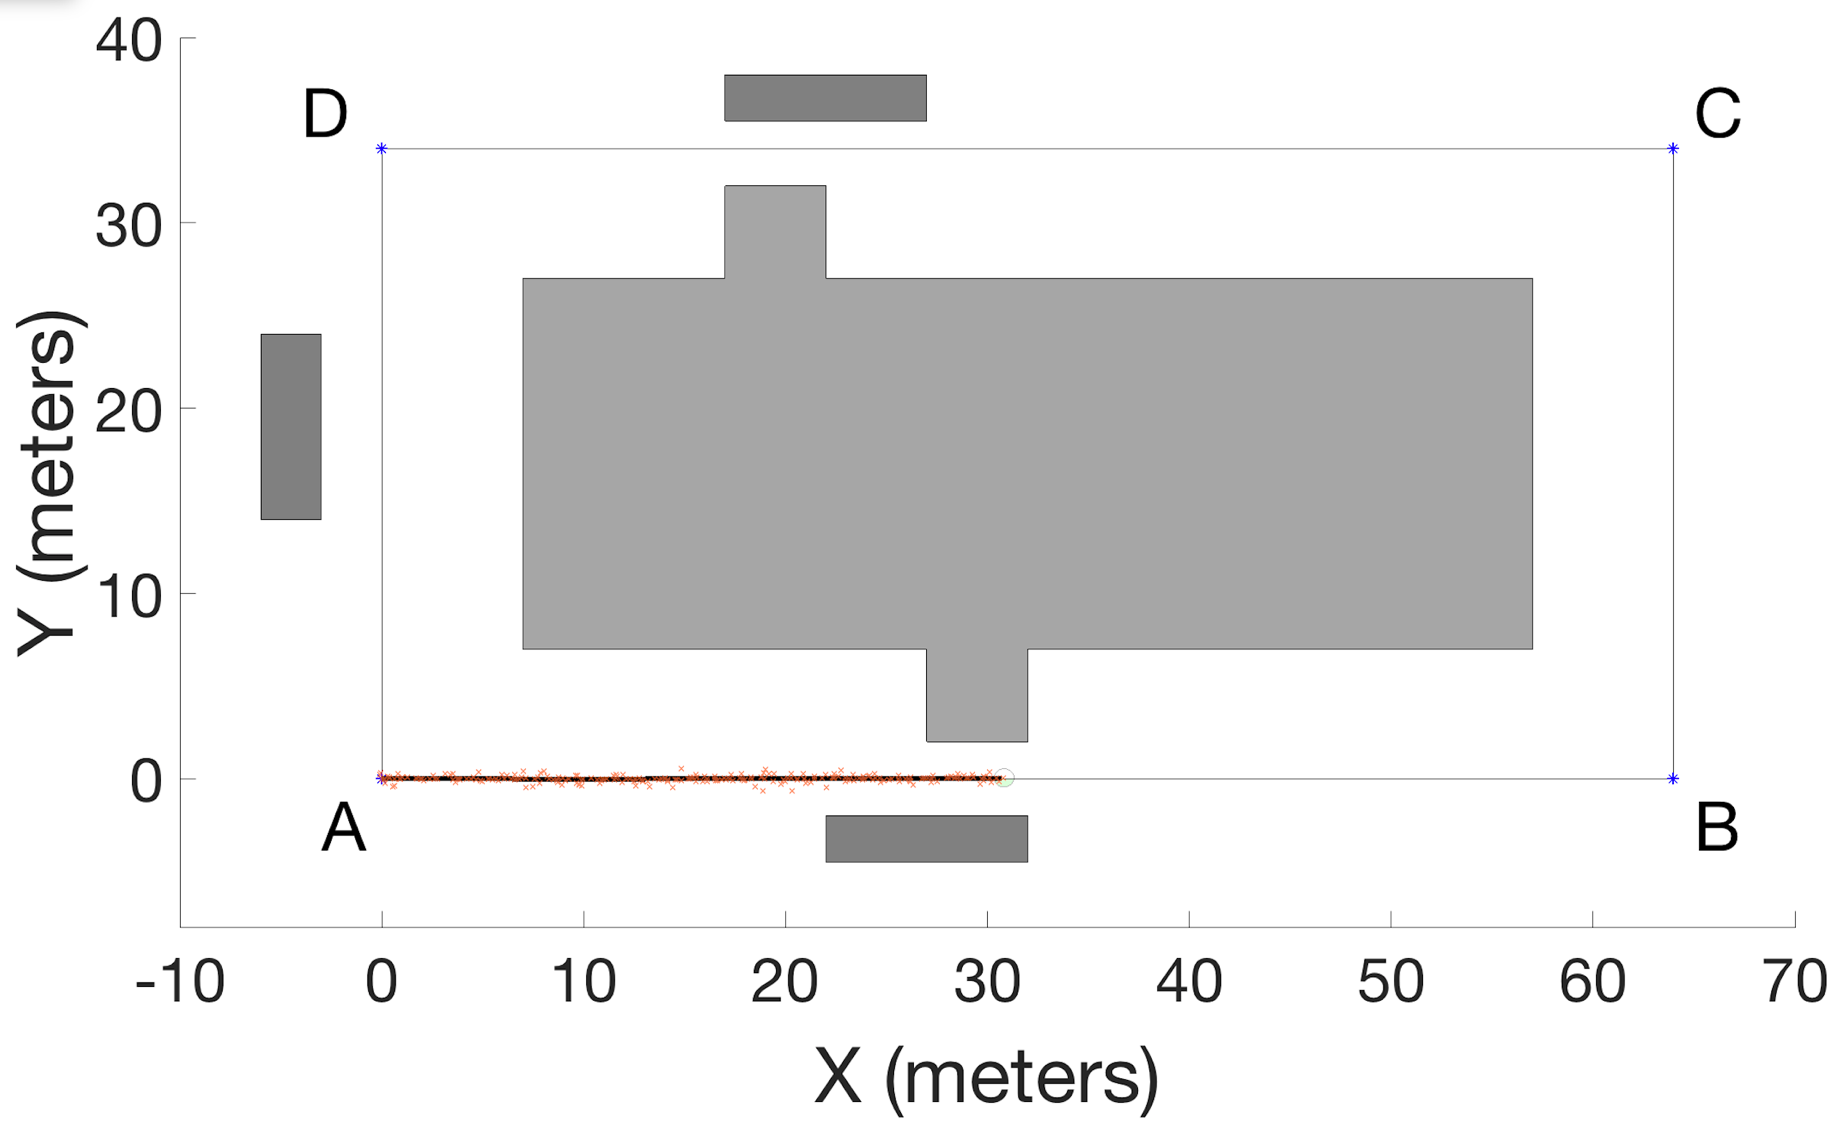
\includegraphics[width = 0.3\textwidth]{Figures/Motion11.png}} &	
\subfigure[\label{fig:low_noise2} ]{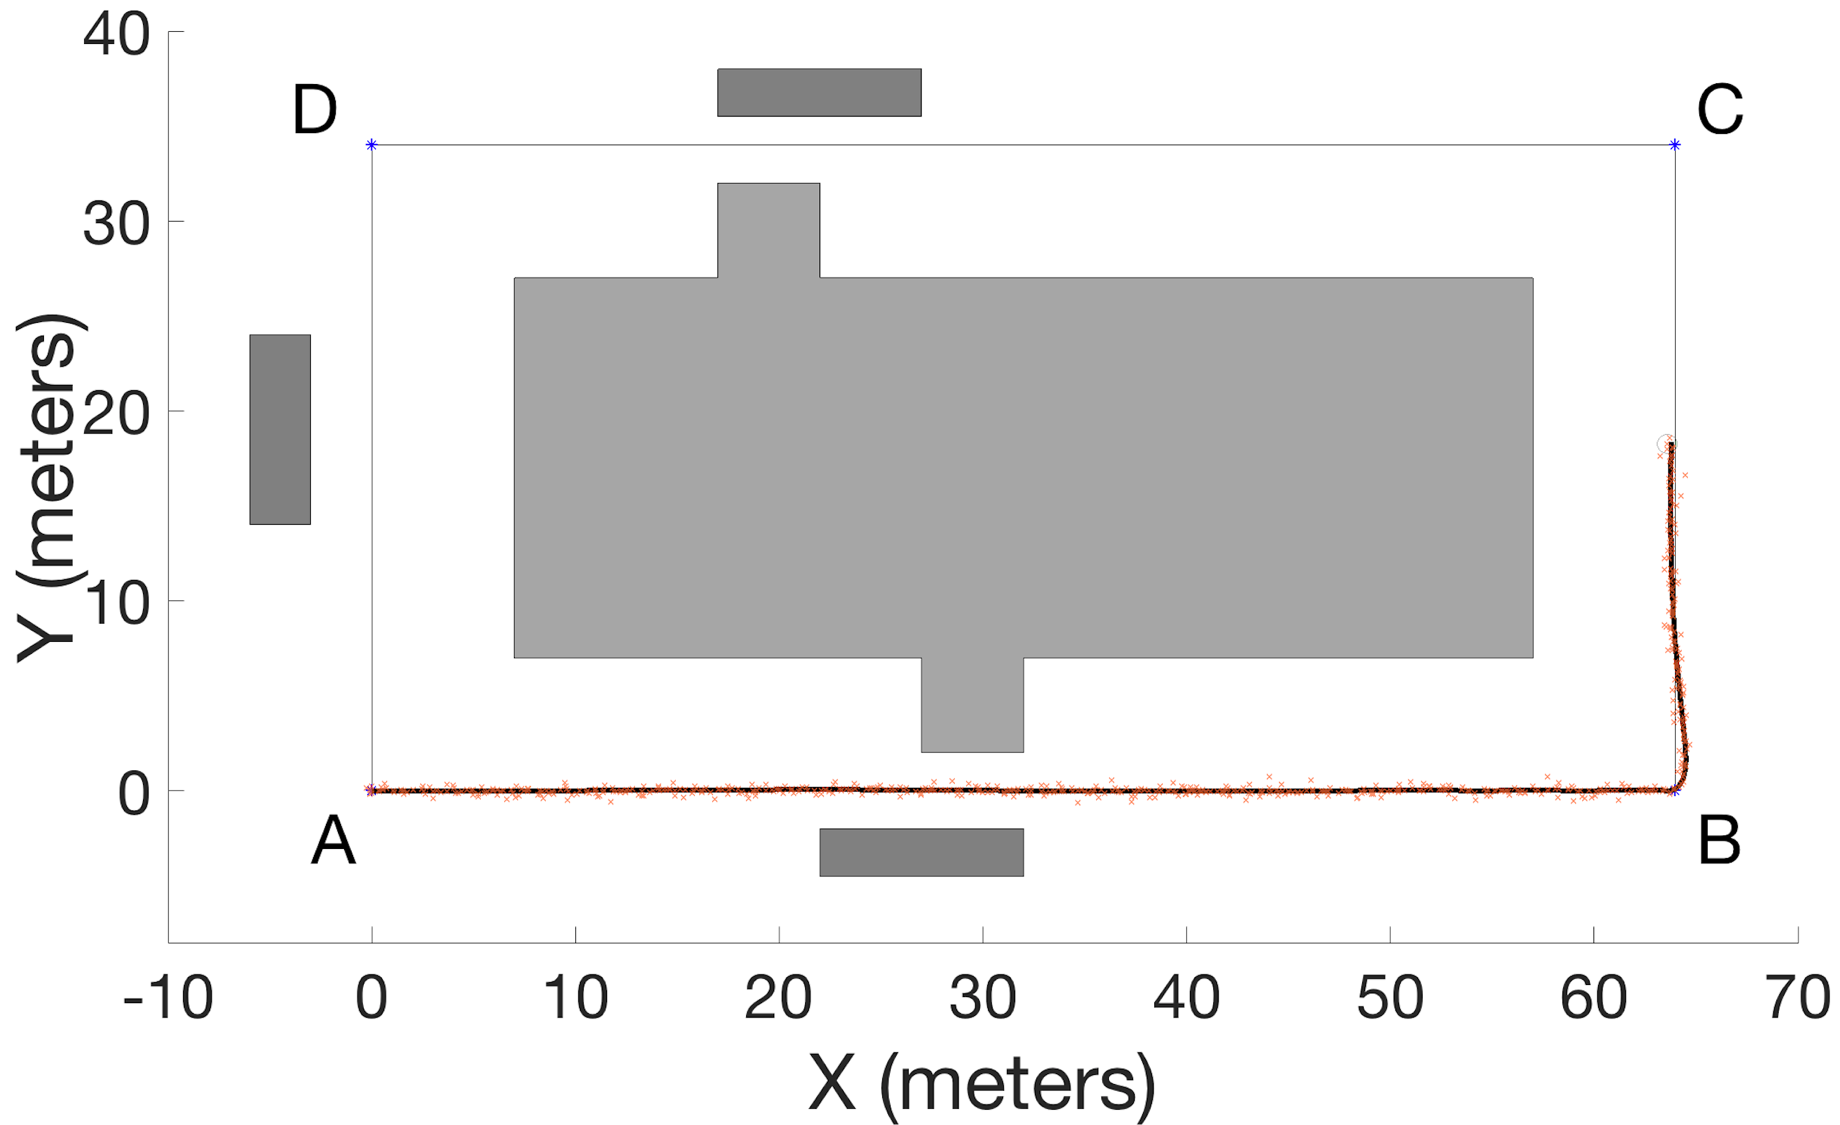
\includegraphics[width = 0.3\textwidth]{Figures/Motion22.png}} &
\subfigure[\label{fig:at_attack} ]{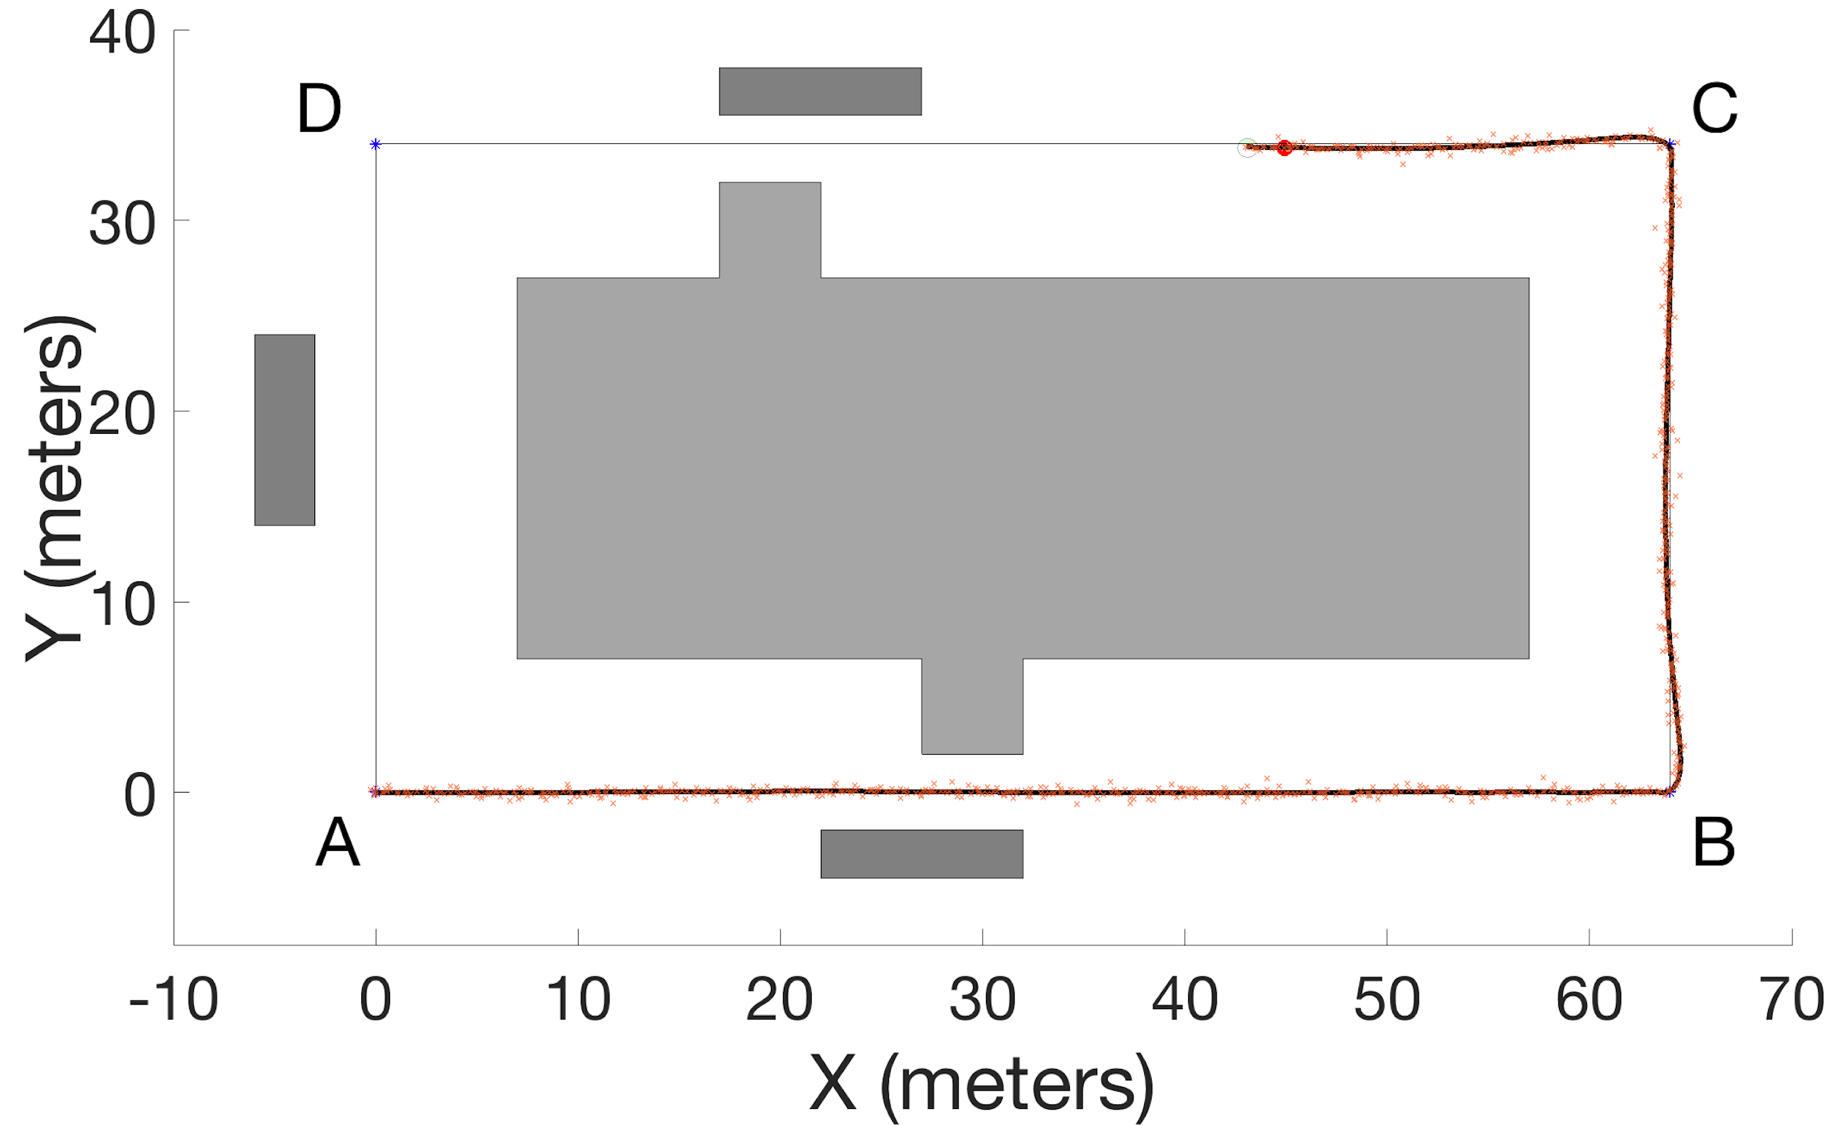
\includegraphics[width = 0.3\textwidth]{Figures/Motion33.png}}
\end{tabular} \\
\begin{tabular}{ccc}
\subfigure[\label{fig:after_detection} ]{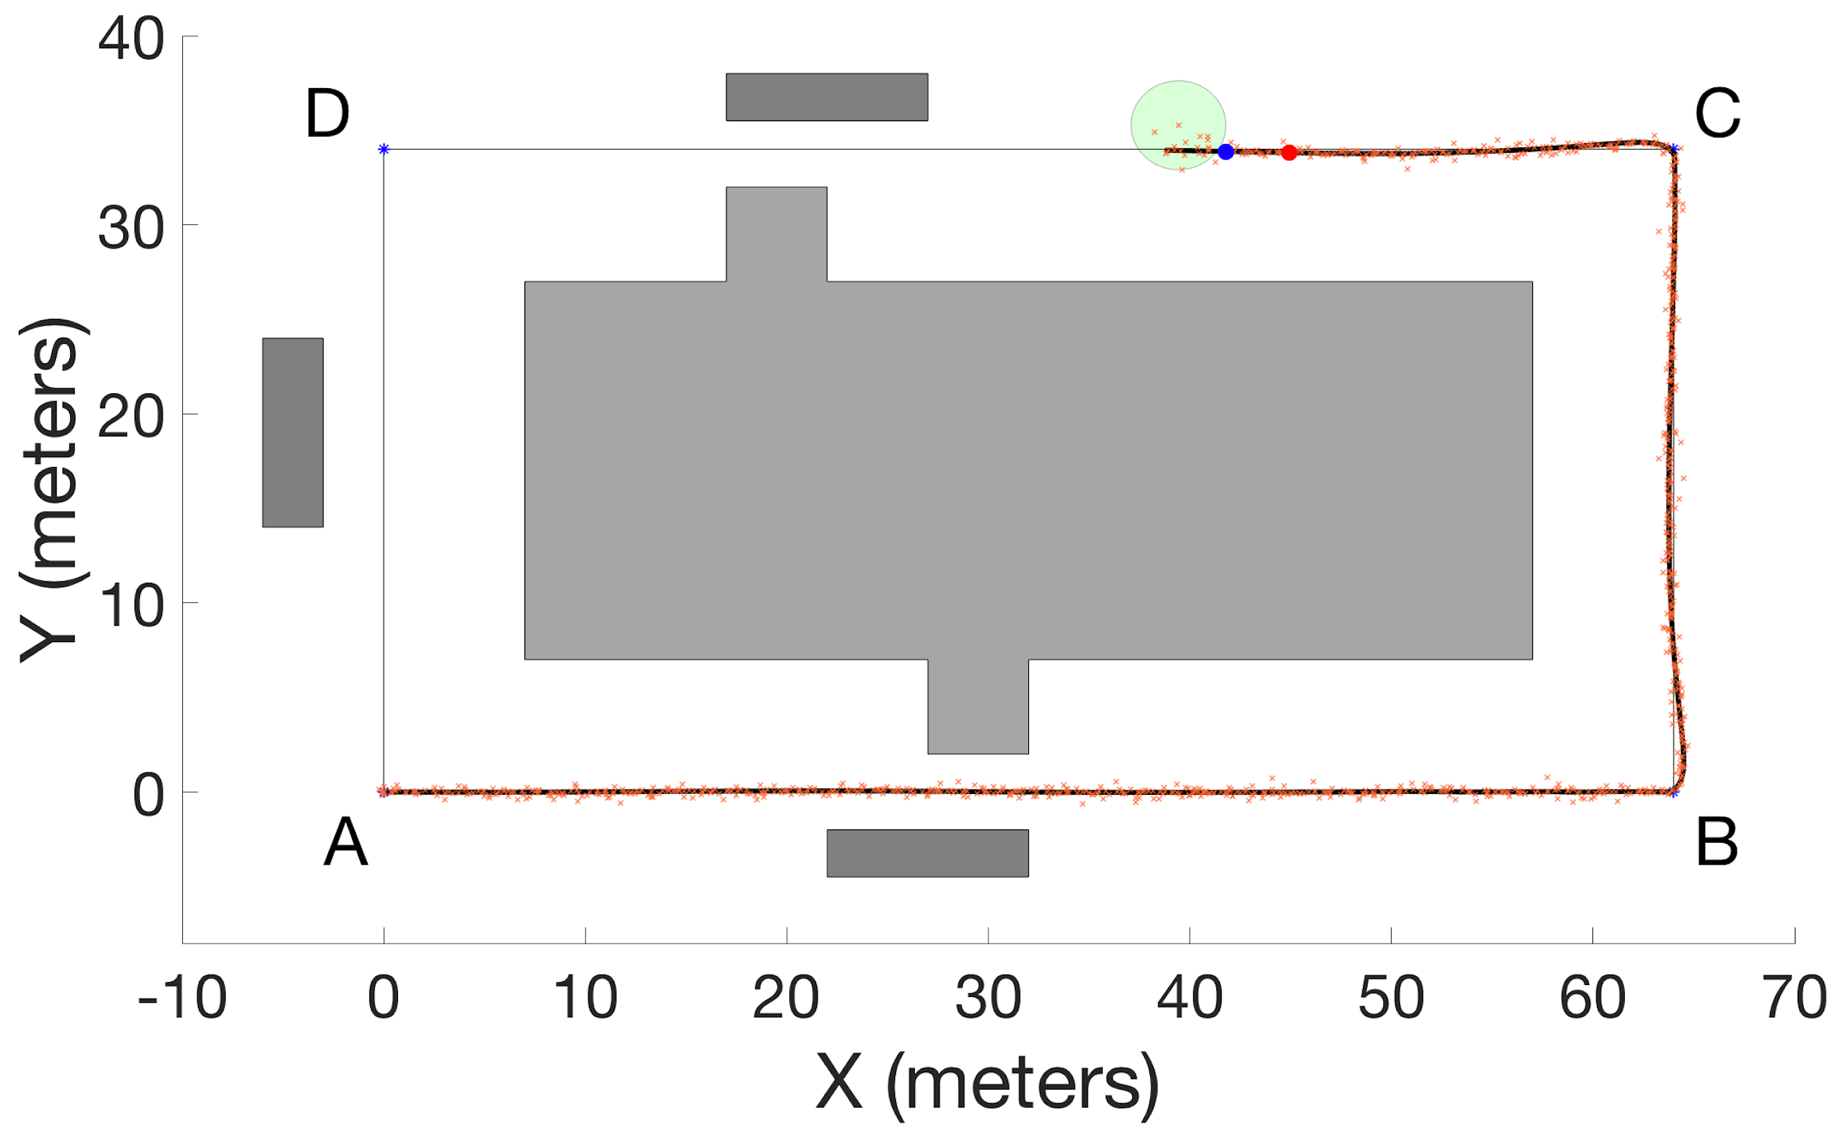
\includegraphics[width = 0.3\textwidth]{Figures/Motion44.png}} &
\subfigure[\label{fig:adapt_region} ]{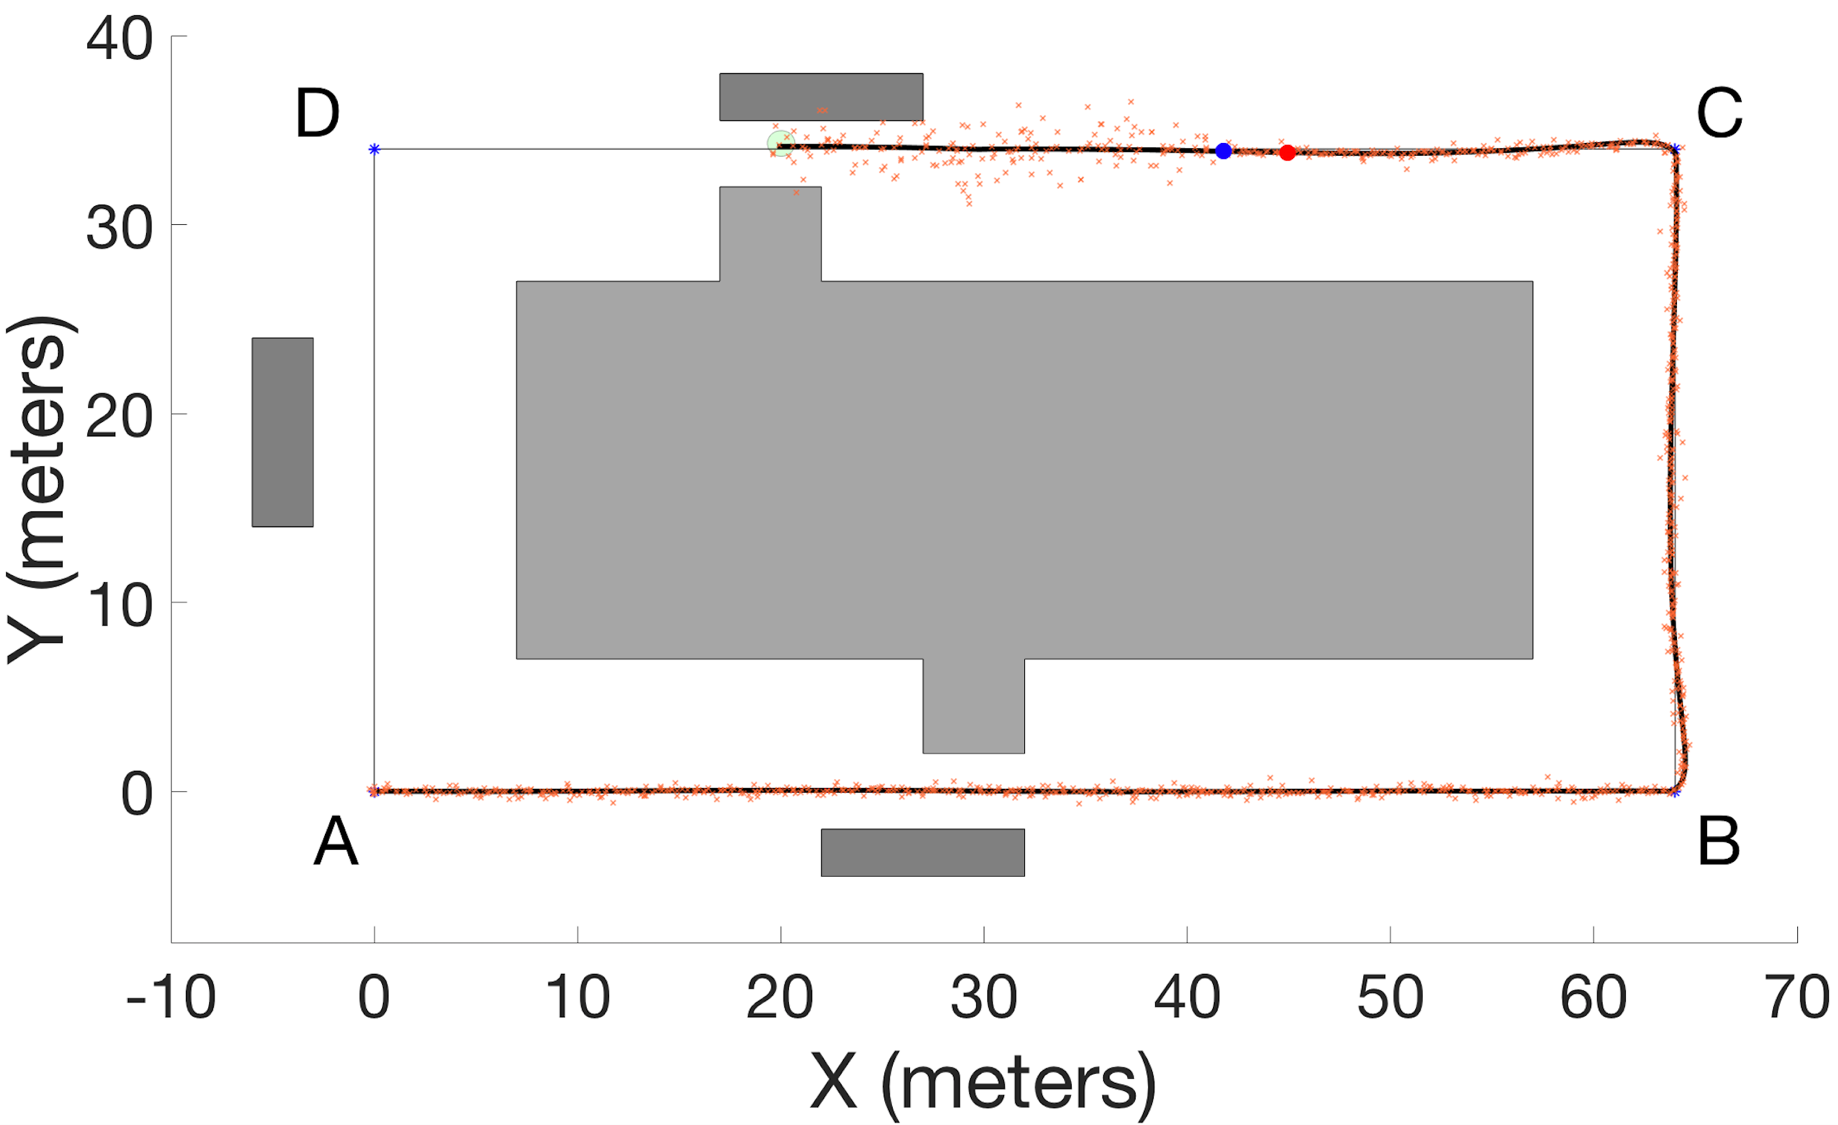
\includegraphics[width = 0.3\textwidth]{Figures/Motion55.png}} & 
\subfigure[\label{fig:continue_motion} ]{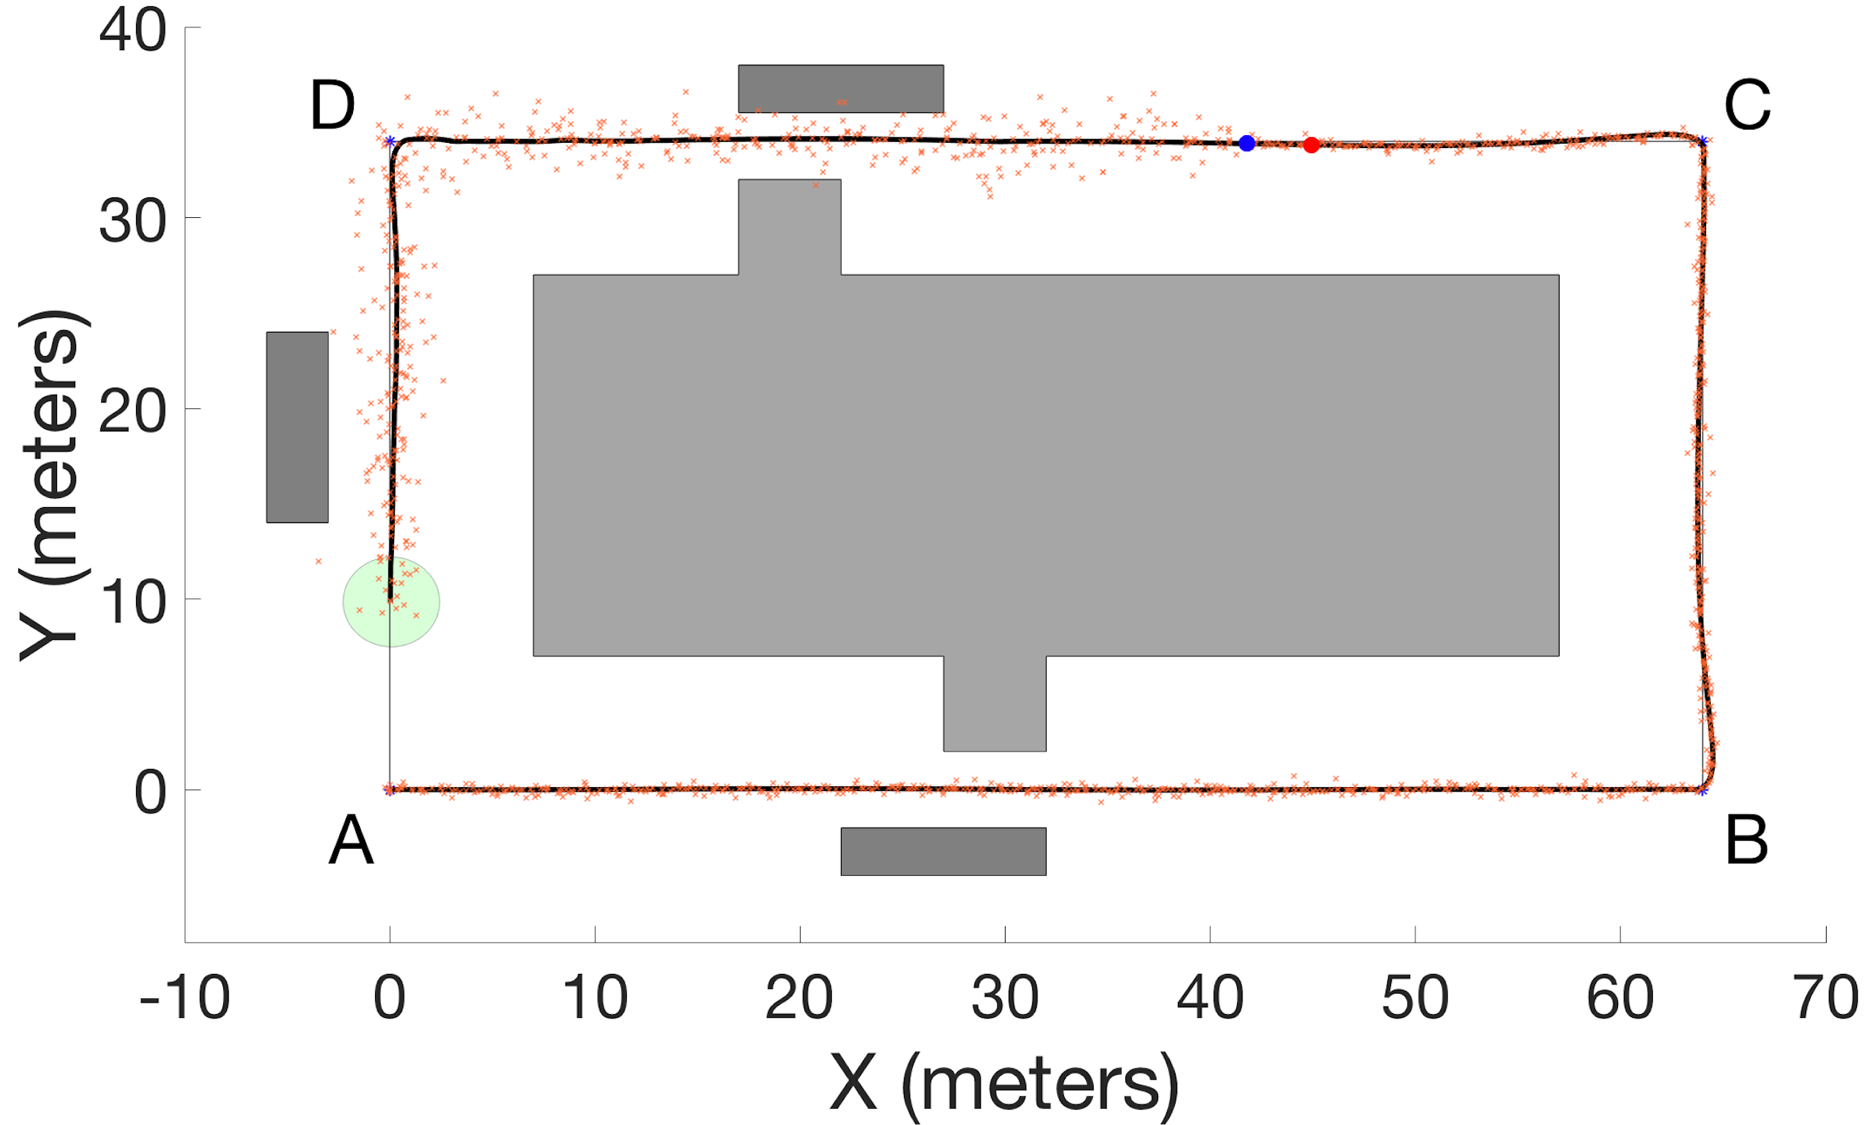
\includegraphics[width = 0.3\textwidth]{Figures/Motion66.png}}
\end{tabular}

\vspace{-8pt}
\caption{ Sequence of snapshot for a vehicle autonomous navigation in a cluttered environment. (b) the vehicle undergoes changes in dynamics. In (c) one of the sensors is spoofed and detected in (d). In (e) the motion planning adaptation technique proposed in Section V.C is deployed slowing down the vehicle when near an obstacle. Finally in (f) the vehicle is able to use its original reference toward the goal.} 
%A comparison in time of a vehicle navigating through an obstacle filled environment. In (a),(b), and (c) the measurement set is uncompromised and the system is only experiencing dynamical changes. Subfigures (d),(e), and (f) are post detection of a sensor attack where the sensor has been removed from the measurement set. Uncertainty is increased with the smaller sensor set, now the vehicle adapts the velocity as it approaches obstacles.}
\vspace{-8pt}
\label{fig:simulation}
\end{figure*}

The case study investigated in this paper is an autonomous unmanned ground vehicle (UGV) navigation under the effects of sensor noise, dynamical changes, and sensor attacks. The vehicle is tasked to travel along a pre-planned trajectory through an obstacle populated environment. 
%We consider a ground vehicle starting at an initial position $\bm{p}(0)=\begin{bmatrix} 0,0 \end{bmatrix}^T$ facing the positive $x$ direction with zero velocity. 
The objective for the UGV is to reach multiple goal points while following a desired trajectory with obstacles of varying distances from the path. The maximum velocity of the vehicle is 3.5m/s and the desired reference velocity is set to 2.5m/s. Three sensors are available to obtain velocity measurements, each with a different level of noise. Throughout the simulation, dynamics are changing affecting the velocity before, during, and after an attack. 

In Fig. \ref{fig:low_noise}, the vehicle is moving along the trajectory with no compromised sensors and far from obstacles. The confidence region is small in this case because all sensors are available and fused together. While all sensors are uncompromised, Fig. \ref{fig:low_noise2} shows a region where the vehicle is undergoing dynamical changes. The confidence region remains unchanged due to the full uncompromised set of sensors. The adaptive controller is maintaining a reference velocity, even while system dynamics are changing. Fig. \ref{fig:at_attack} shows vehicle position at the starting time of a ramped sensor attack. Detection has not occurred due to the attack is within the error threshold $\delta(k)$. In Fig. \ref{fig:after_detection} the spoofed sensor is detected and removed leaving a smaller set of available sensors with higher uncertainty. As demonstrated in the figure, the confidence region grows in size due to the changes in uncertainty. Because obstacles are still well outside of the bounds, the vehicle can continue navigating at its desired velocity. Fig. \ref{fig:adapt_region} shows the confidence region shrinking in size when the vehicle navigates near obstacles of closer distances. More data points are used to improve this estimation, while the velocity is reduced to lessen state estimation uncertainty as discussed in Section \ref{sec:estimation_confidence}. Once the vehicle is past the obstacles that are at close distances, shown in Fig. \ref{fig:continue_motion}, the vehicle is able to move freely again at its desired reference velocity. The confidence region remains at a much larger radius due to the smaller set of available sensors. Animations for the simulations presented above can be found at https://www.bezzorobotics.com/pb-acc19.

% \begin{figure}
% \vspace{1pt}
% %\centering
% 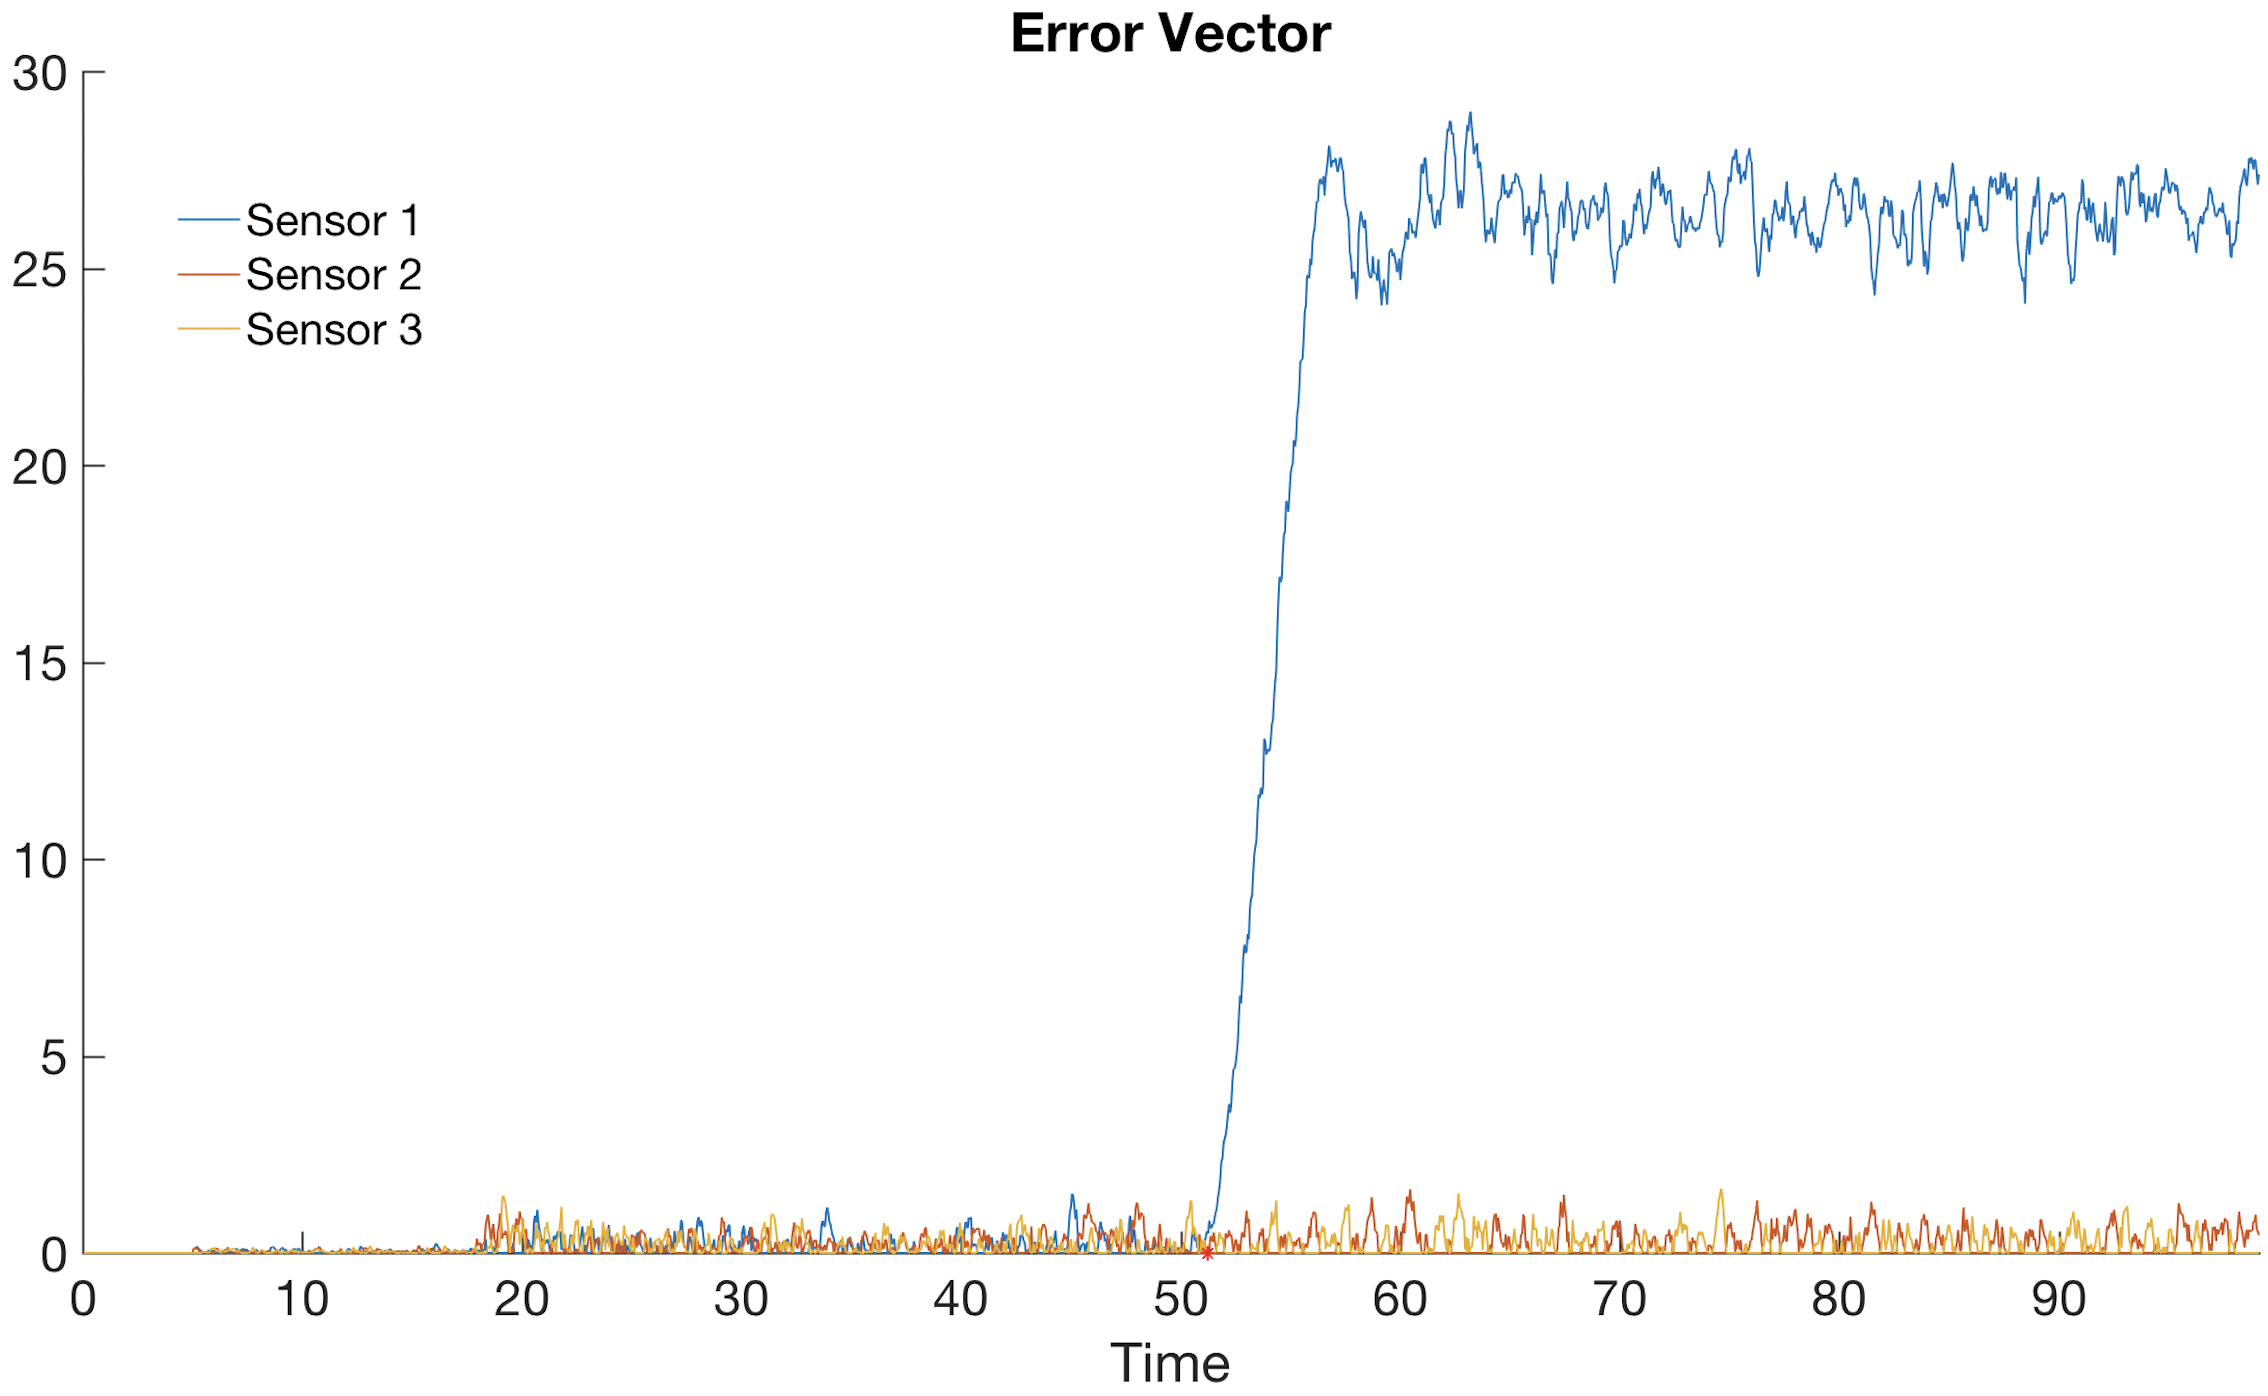
\includegraphics[width=0.48\textwidth]{Figures/Error_vector.png}
% \caption{The error vector is computing magnitudes of error for each of the sensors. As a sensor's error reaches a threshold, the sensor will be removed from the system.}
% \label{fig:sensor error}
% \end{figure}

\begin{figure}[ht]
\vspace{-8pt}
\begin{tabular}{c}
\subfigure[\label{fig:total_velocity} ]{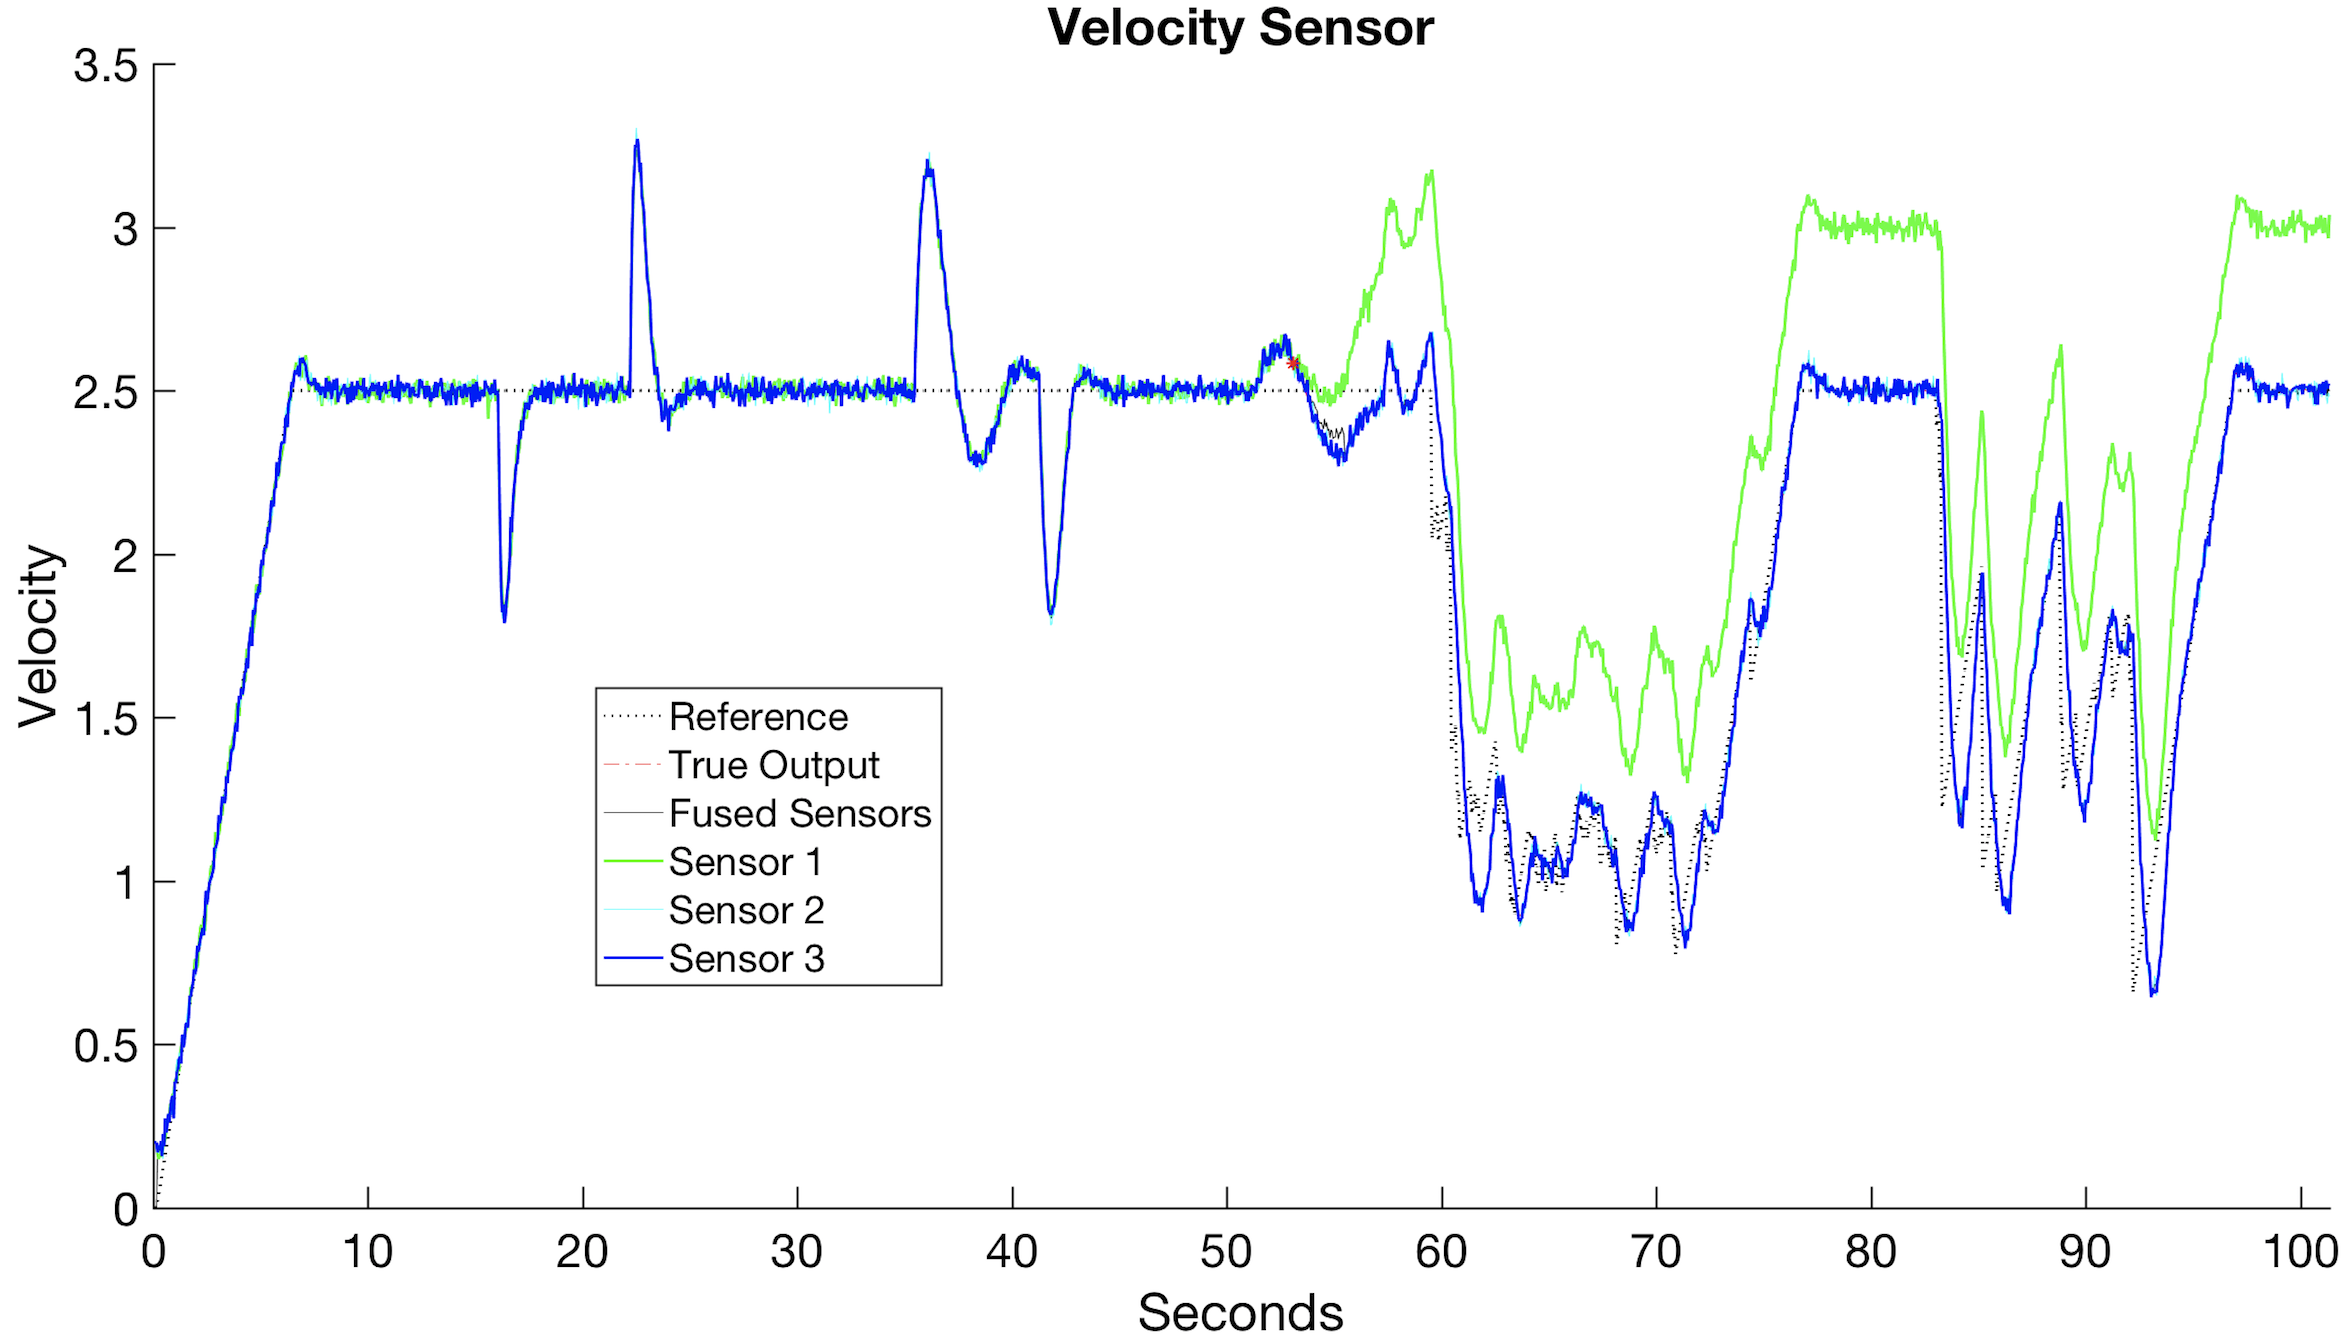
\includegraphics[width = 0.45\textwidth]{Figures/Velocities.png}} 
\end{tabular} \\
\begin{tabular}{c}
\subfigure[\label{fig:total_input} ]{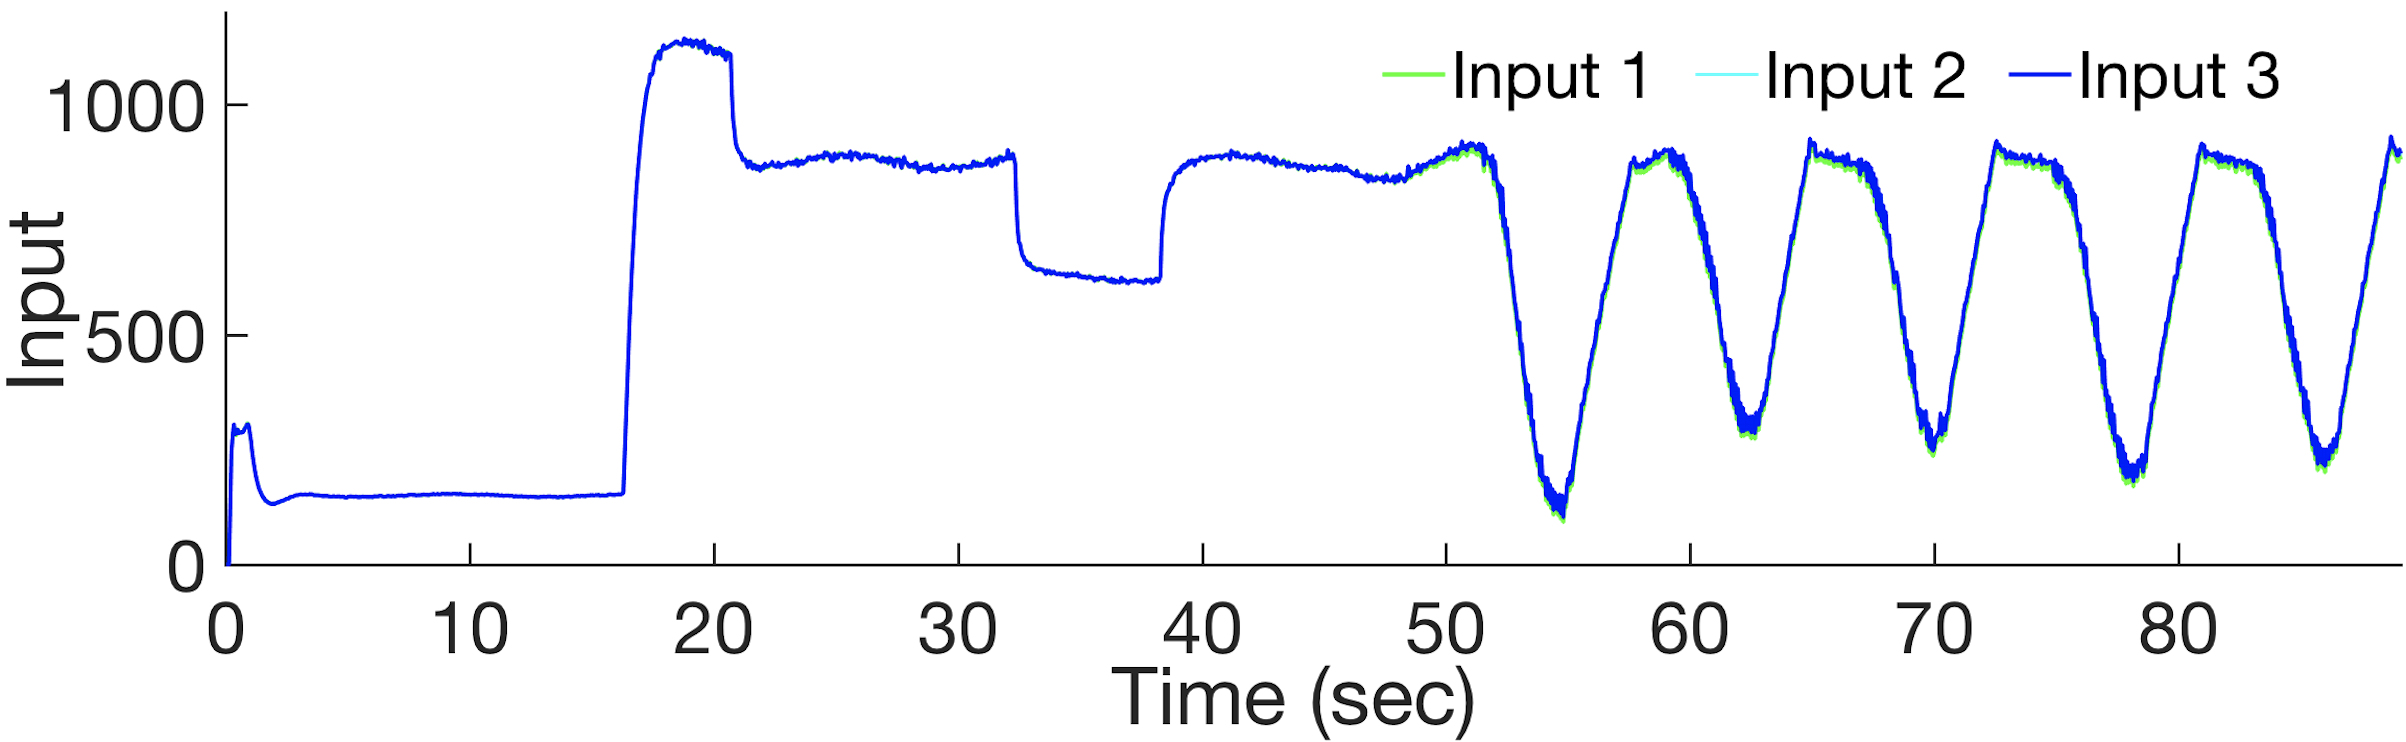
\includegraphics[width = 0.45\textwidth]{Figures/Total_Inputs.png}} 
%\vspace{-10pt}
\end{tabular}
\vspace{-7pt}
\caption{(a) Comparison between velocity measurements and the reference during dynamical changes and sensor attacks for the case depicted in Fig. \ref{fig:simulation}; (b) the three inputs associated to each sensor subsystems with the attacked sensor input different from the other non-spoofed sensors.}
%The velocity measurements in \ref{fig:total_velocity} show the system experiencing dynamical changes and a sensor attack. Subsystem inputs in \ref{fig:total_input} reflect the dynamical changes between Goal points A and C, and the subsystem input of the corresponding spoofed sensor diverges from the other inputs.}
\label{fig:Total_vel_input}
 \vspace{-5pt}
\end{figure}

In Fig. \ref{fig:Total_vel_input}, the velocity measurements and their inputs over the entire simulation are displayed. During the time frame between Goals A and C, dynamical changes occur temporarily affecting the velocity tracking. After Goal C, a spoof on Sensor 1 causing it diverge from the other sensors. The detector removes the compromised sensor, allowing the system to maintain reference tracking. As explained above, the velocity is automatically reduced when the vehicle passes near closer obstacles to allow more data samples and more precise state estimation.




% \begin{figure}[h!]
% \centering
% \begin{tabular}{cc}
% \subfigure[\label{fig:MRAC_tracking} ]{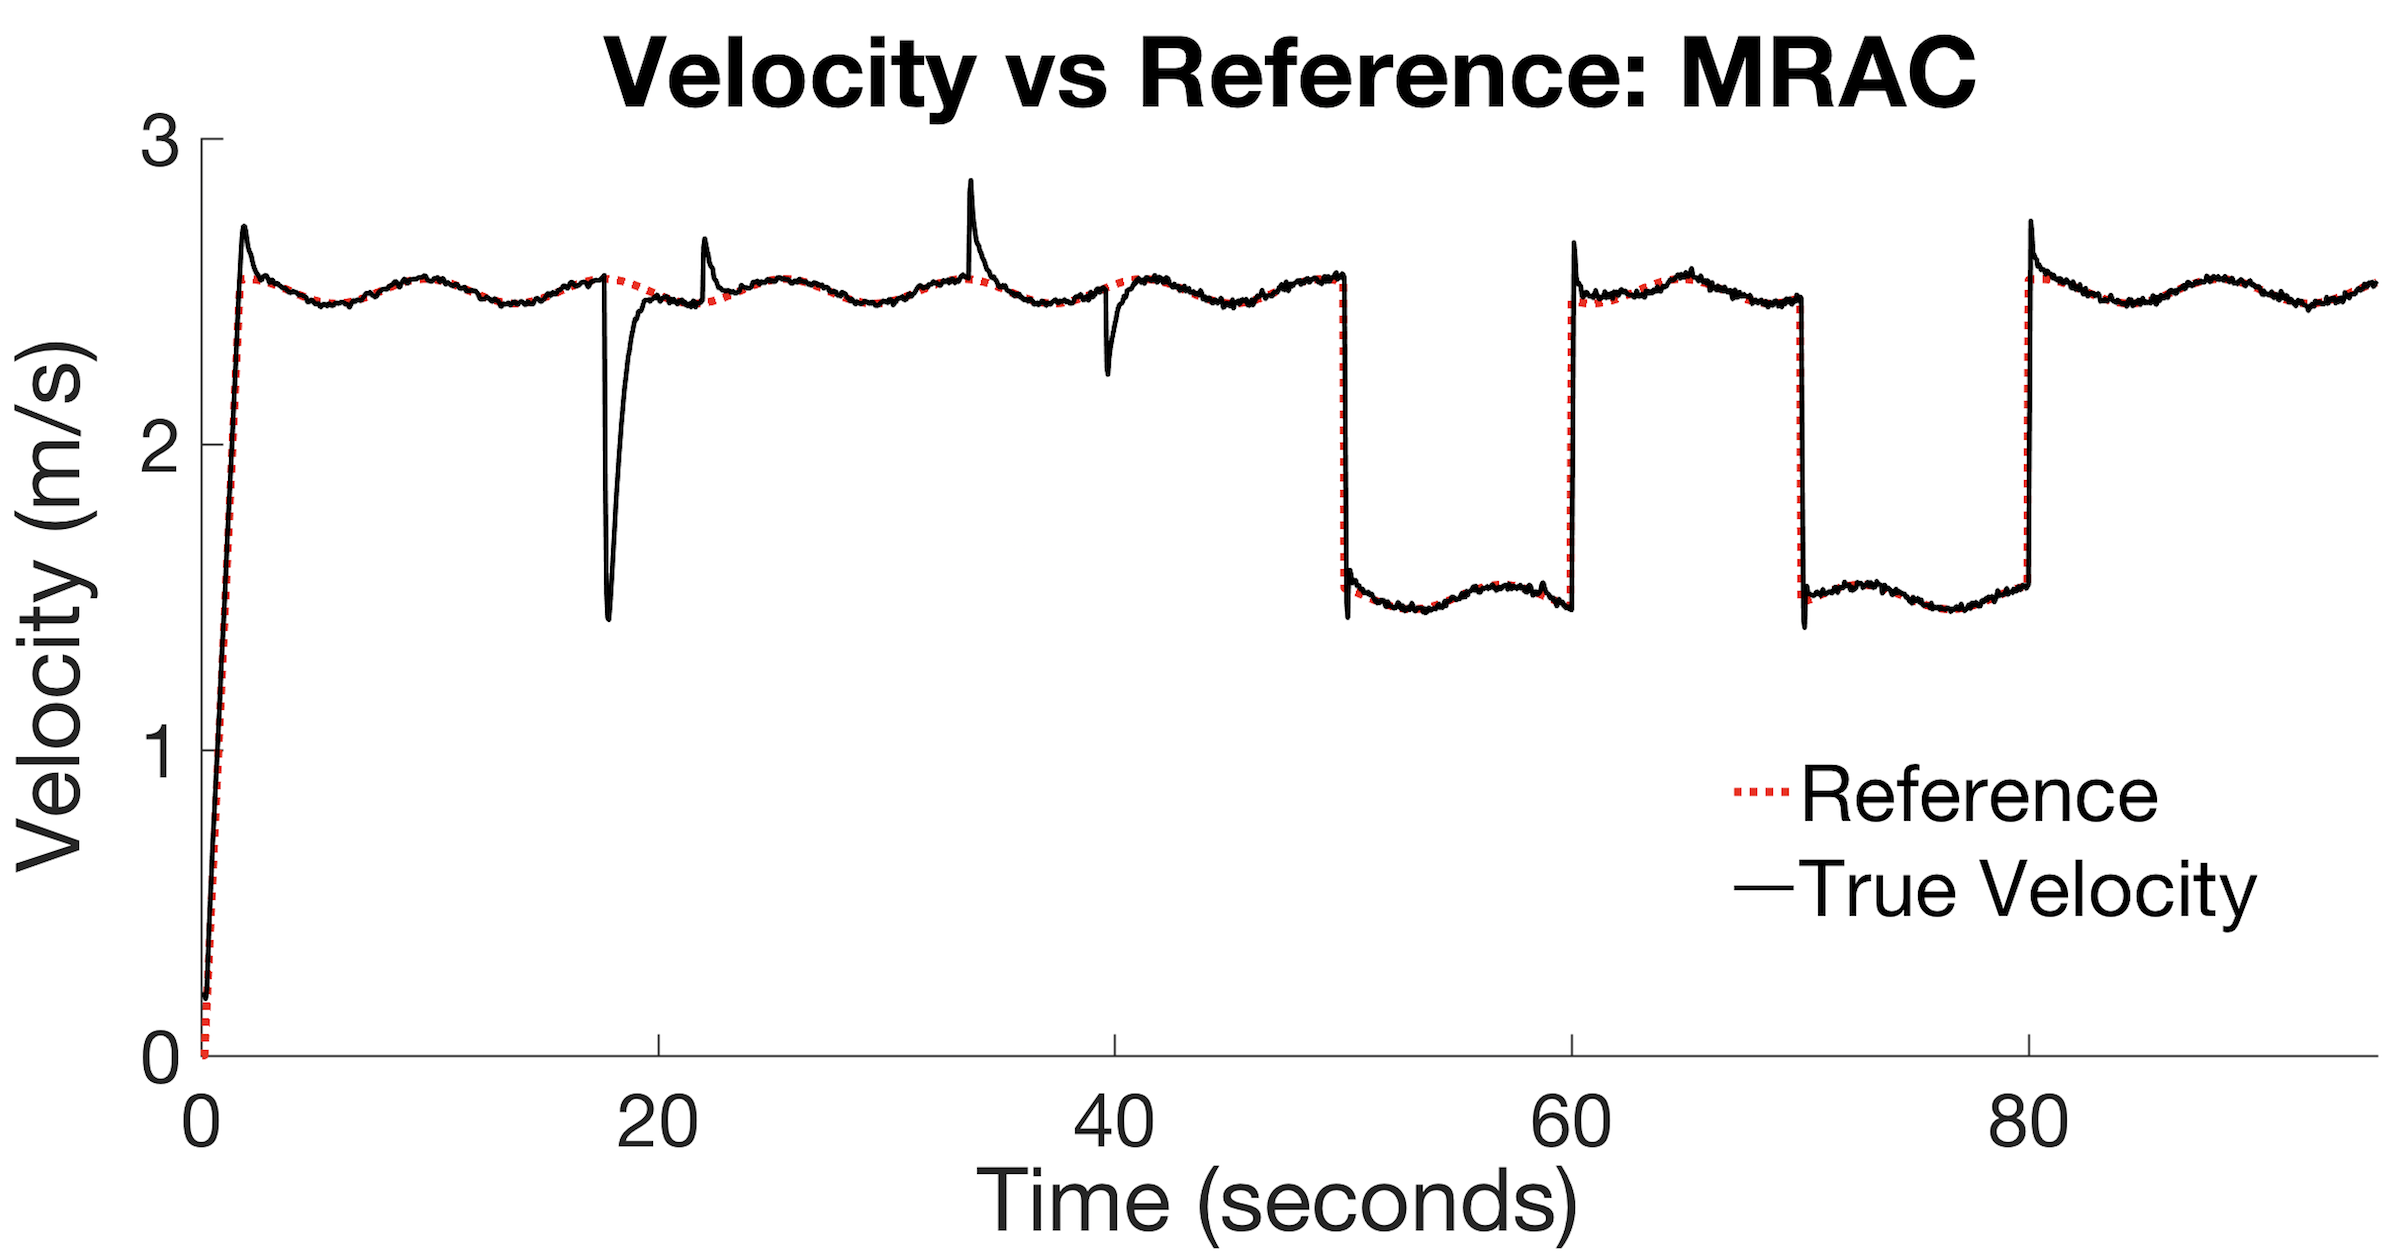
\includegraphics[width = 0.22\textwidth]{Figures/VelocityTracking_MRAC.png}} & 
% \subfigure[\label{fig:PID_tracking} ]{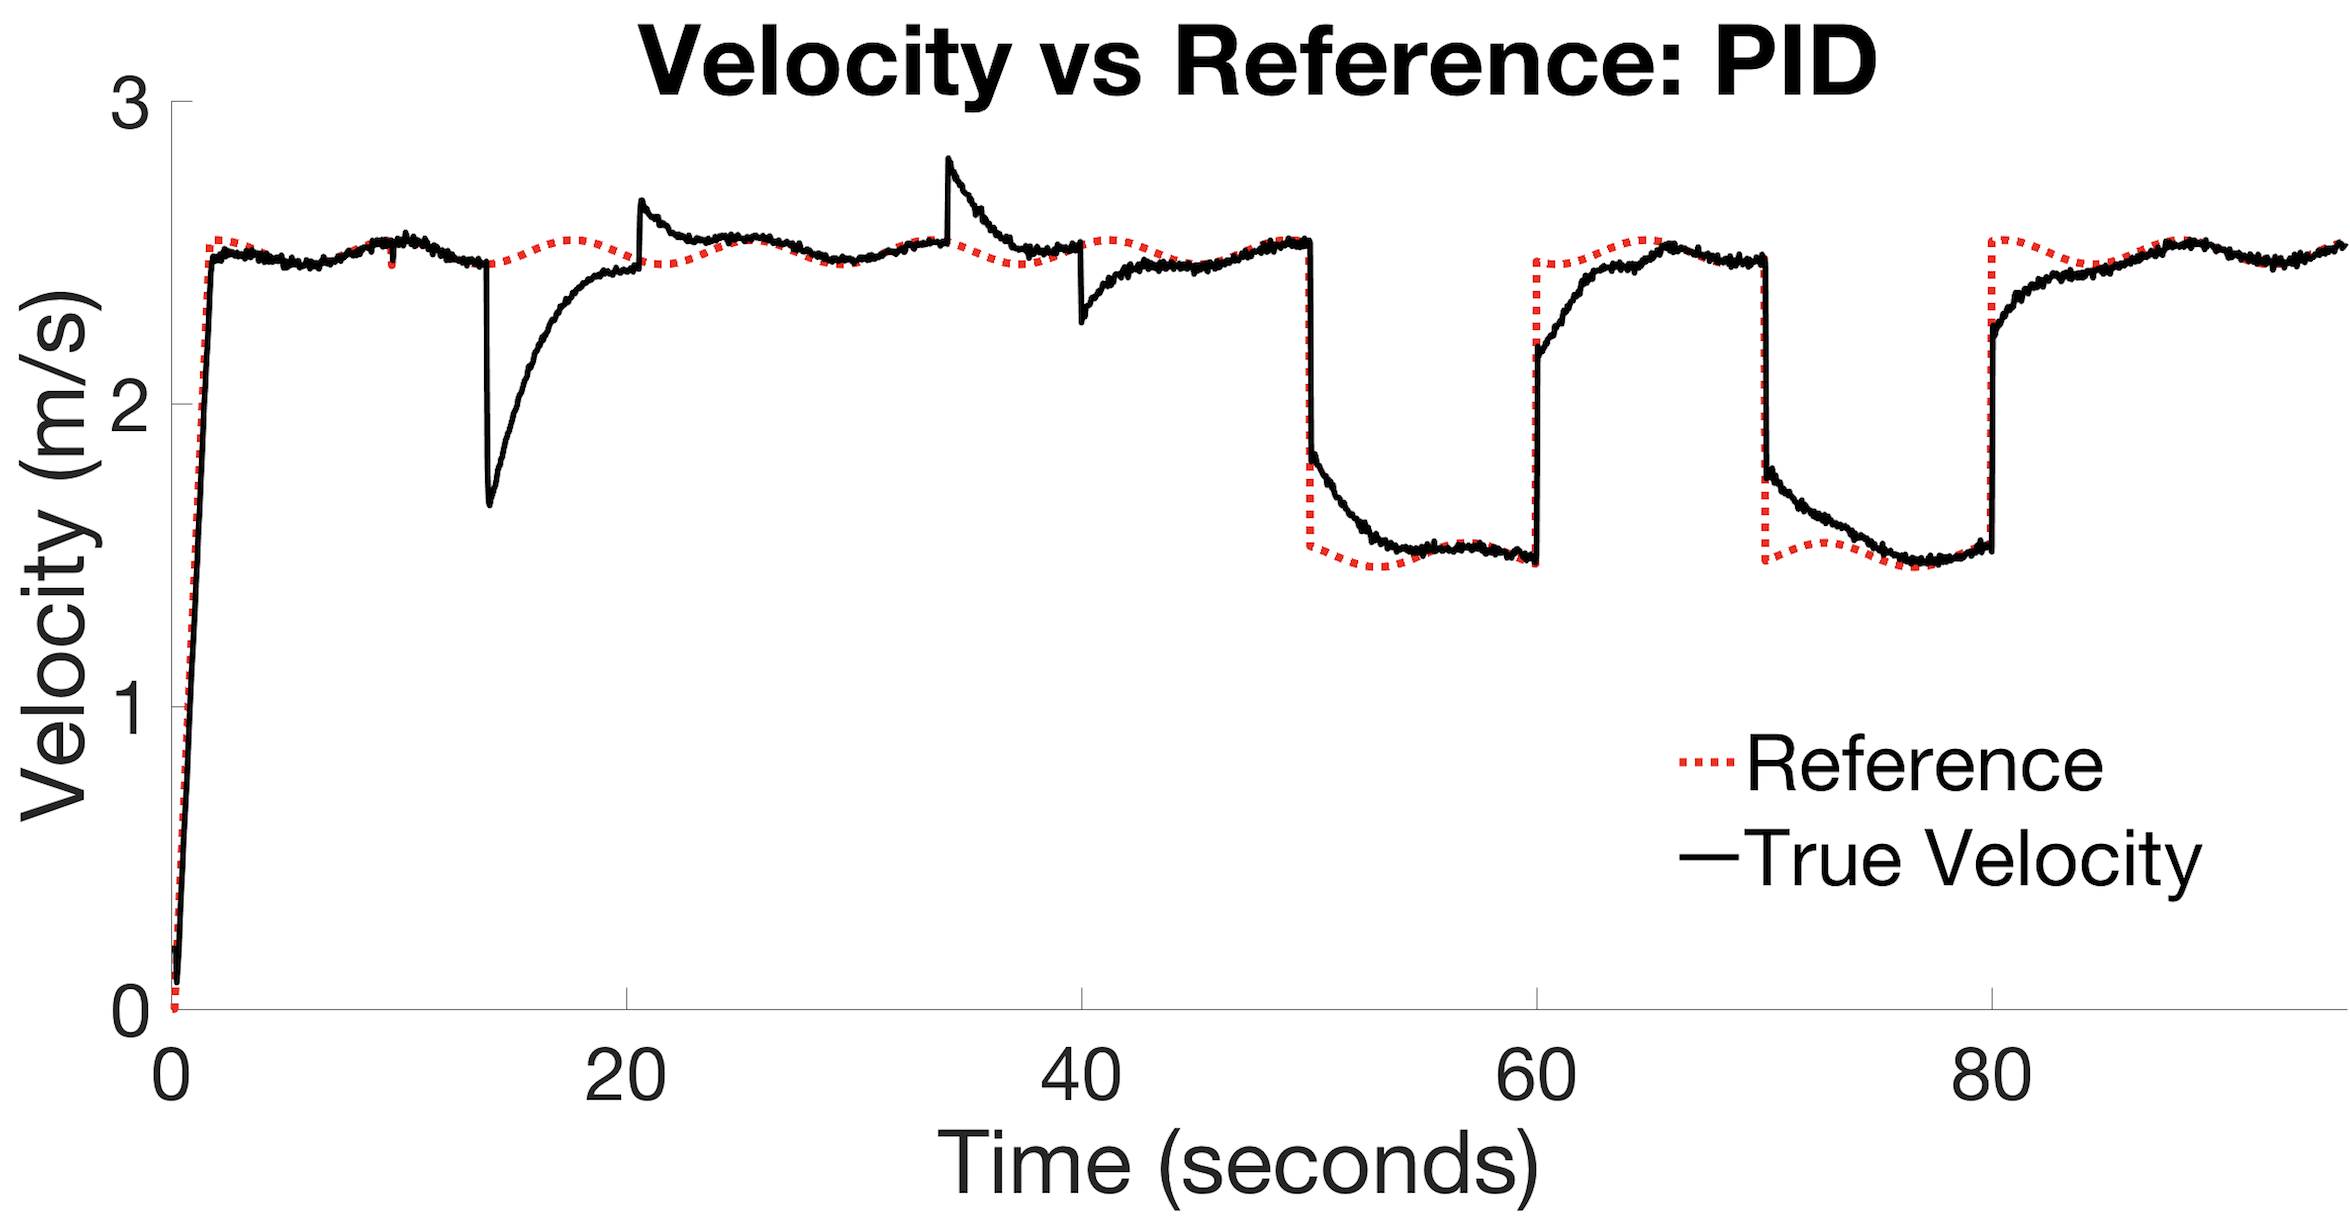
\includegraphics[width =0.22\textwidth]{Figures/VelocityTracking_PID.png}}
% \end{tabular}
% \label{fig:ControllerComparisons}
% \caption{A performance comparison between the model reference adaptive controller (MRAC) vs Proportional-Integral-Derivative (PID) controller tuned for the initial model.}
% \end{figure}

% A comparison of control performance in Figure \ref{fig:ControllerComparisons} shows the benefits of the adaptive controller. As dynamics change away from the initial model, the PID controller loses control performance in which the tracking convergence is degraded.




% \begin{figure}
% \vspace{1pt}
% %\centering
% 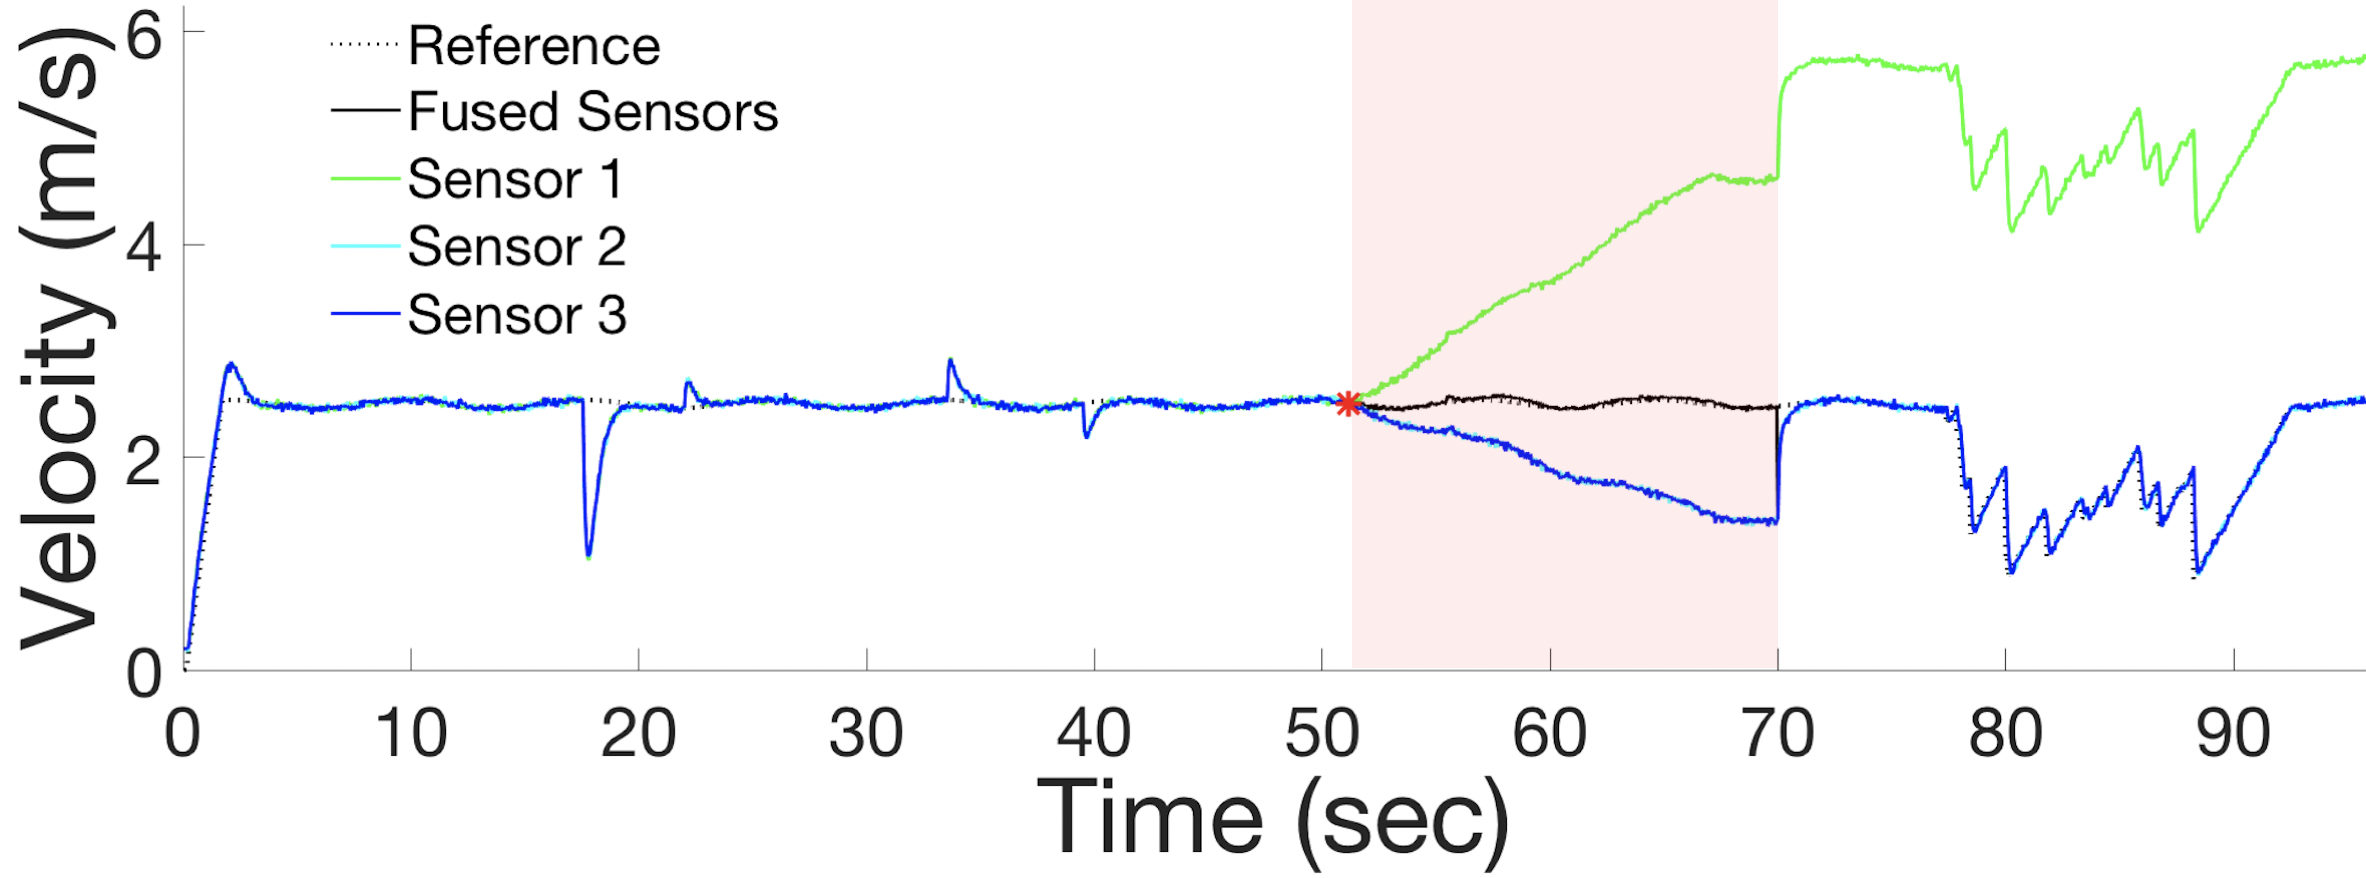
\includegraphics[width = 0.48\textwidth]{Figures/NoDetection_Vel.png}
% \caption{A demonstration of an attack with the detector not operating for a period of time during an attack. As the right shaded region ends, the detector is turned on and the sensor is removed.}
% \label{fig:NoDet_Vel}
% \end{figure}

% Figure \ref{fig:NoDet_Vel} shows a time frame of the detector turned off, where an attacker is free to compromise the system. A ramp attack is performed, slowly pushing a sensor away from the true value. The red shaded region is the time frame the attack occurred without the attack detector operating. 


\begin{figure}
\vspace{-5pt}
\begin{tabular}{cc}
\subfigure[\label{fig:error_comp1} ]{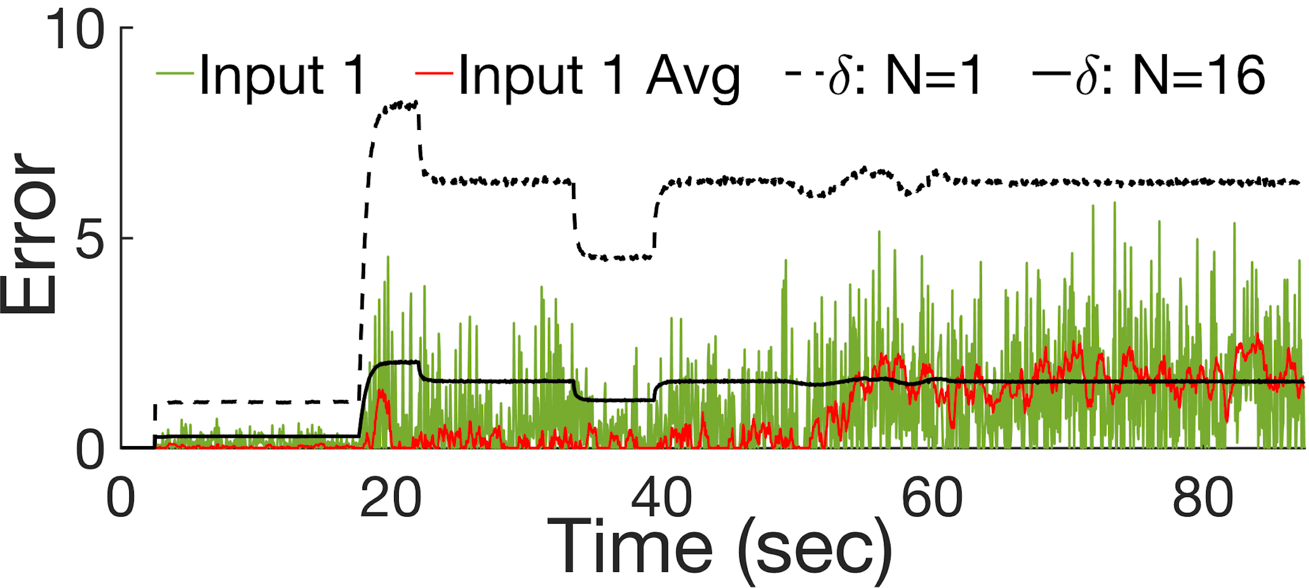
\includegraphics[width = 0.22\textwidth]{Figures/ErrorComparison11.png}} &	
\subfigure[\label{fig:error_comp2} ]{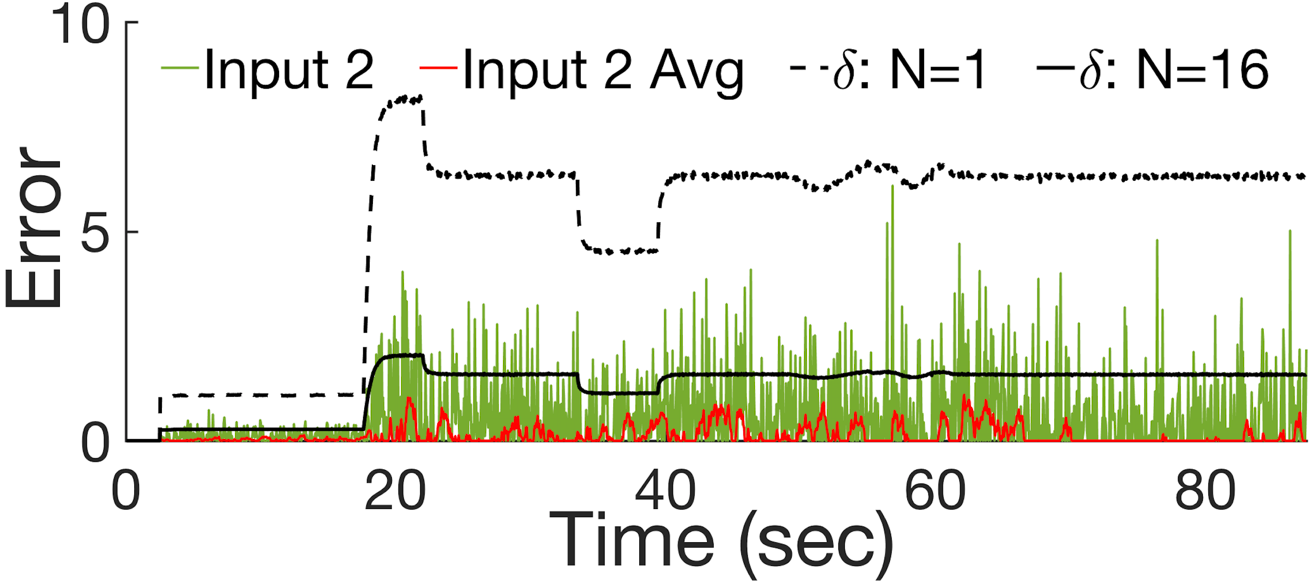
\includegraphics[width = 0.22\textwidth]{Figures/ErrorComparison22.png}}
\end{tabular} 
\vspace{-10pt}
\caption{Stealthy attack case study. (a) sensor 1 is compromised and not detectable in one time step (green line) but becomes visible considering $N_p=16$ steps (red line) using the approach in \eqref{eq:max_error2}. (b) shows the error associated with sensor 2 which was uncompromised.}
%In the case of an adversary performing a stealthy attack within the noise profile, using a value of $N_p>1$ from \eqref{eq:max_error2} reduces the detection error threshold \eqref{eq:delta} for better visibility. }
\label{fig:Stealthy_Attack}
\vspace{-10pt}
\end{figure}

Stealthy attacks within the sensor noise profile can be detected by using more input values to reduce the noise threshold $\delta$. The case in Fig. \ref{fig:Stealthy_Attack}, leveraging the discussion in Section \ref{sec:Res_adapt_control}, demonstrates the attack on Sensor 1 is detected when using $N_p=16$ input values, but would have never been detected when $N_p=1$ as the error stayed below the error threshold $\delta$.



\end{section}